\documentclass[12pt]{article}
\usepackage[utf8]{inputenc}
\usepackage[T1]{fontenc}
\usepackage[english]{babel}
\usepackage{ifpdf,newtxtext,newtxmath} 
\usepackage{array,graphicx,dcolumn,multirow,hevea,abstract,hanging,fancyhdr,float}
\makeatletter
\newcommand{\checkheight}[1]{%
  \par \penalty-100\begingroup%
  \setbox8=\hbox{#1}%
  \setlength{\dimen@}{\ht8}%
  \dimen@ii\pagegoal \advance\dimen@ii-\pagetotal
  \ifdim \dimen@>\dimen@ii
    \break
  \fi\endgroup}
\makeatother
%\usepackage{float}

\topmargin=-.3in \oddsidemargin=.3in \evensidemargin=.3in \textheight=9in \textwidth=6in
\pagestyle{fancy} 

\renewcommand{\headrulewidth}{0pt} % Removing the header lines
\renewcommand{\footrulewidth}{0pt}

\usepackage[labelfont=sc,textfont=sf]{caption}
\usepackage[hyperfootnotes=false,breaklinks=true]{hyperref} % was dvipdfmx
\urlstyle{rm}
\usepackage[hyphenbreaks]{breakurl}


% DO NOT USE ADDITIONAL PACKAGES unless you make sure they work with Hevea.
% You may define new commands, but these may cause other troubles, so try to avoid it.

% FOR BIBTEX USERS (Bibtex is not recommended, but we can use it):
% \usepackage{natbib} % must come afer hypperref
% in references: \bibliographystyle{apalike3} \setlength{\bibsep}{0pt} \bibliography{WHATEVER}
% download http://journal.sjdm.org/apalike3.bst
\usepackage{booktabs} % \toprule \midrule \bottomrule \cmidrule(lr){a-b}
% define centered and ragged columns:
\newcolumntype{L}[1]{>{\raggedright\arraybackslash }p{#1}} % can use m{}
\newcolumntype{C}[1]{>{\centering\arraybackslash }p{#1}}
\newcolumntype{R}[1]{>{\raggedleft\arraybackslash }p{#1}}
\newcolumntype{d}[1]{D{.}{.}{#1}} % d{3.2} for 3 places on l, 2 on r
\newcommand{\mc}{\multicolumn}
\setlength\tabcolsep{1mm}
\setlength\columnsep{5mm}
\setlength\abovecaptionskip{1ex}
\setlength\belowcaptionskip{.5ex}
\setlength\belowbottomsep{.3ex}
\setlength\lightrulewidth{.04em}
\renewcommand\arraystretch{1.2}
\renewcommand{\topfraction}{1}
\renewcommand{\textfraction}{0}
\renewcommand{\floatpagefraction}{.9}
% \renewcommand{\baselinestretch}{1.00} \large\normalsize % for fixing spaces
\widowpenalty=1000
\clubpenalty=1000
\setlength{\parskip}{0ex}
\let\tempone\itemize
\let\temptwo\enditemize
\let\tempthree\enumerate
\let\tempfour\endenumerate
\renewenvironment{itemize}{\tempone\setlength{\itemsep}{0pt}}{\temptwo}
\renewenvironment{enumerate}{\tempthree\setlength{\itemsep}{0pt}}{\tempfour}

\usepackage{xcolor,listings}
\usepackage{textcomp}
\usepackage{wrapfig}
\usepackage{authblk}
\lstset{upquote=true}
%%%%%%%%%%%%%%%%%%%%%%%%%%%%%%%%%%%%%%%%%%%%%%%%%%%%%%%%%%%%%%%%%%%%%
\setcounter{page}{1} % start with first page

\title{Foreign Media Influence on the South Pacific Environment}

\author{
Derek Lilienthal\thanks{California State University, Monterey Bay, Seaside CA 93955}\;\,\thanks{dlilienthal@csumb.edu}\\{\small Advisor: Dr. Elizabeth Gooch\thanks{Naval Postgraduate School, Monterey CA 93943}\;\,\thanks{elizabeth.gooch@nps.edu}}}




\date{\small Febuary 2021} % leave empty
\begin{document} % goes here

\begin{htmlonly}
\href{\jref}{\jhead}, \jdate, pp.\
\end{htmlonly}

\maketitle

\begin{abstract}

In this research, we quantify foreign actors media activities in the South Pacific involving an environmental theme. We use the GDELT (Global Database of Events, Language, and Tone) data set to compare the tones of articles produced by Western, Chinese, and South Pacific (Local) media sources that involve an environmental theme and when a great power (United States, China, Australia, New Zealand, Japan, and Russia) is involved as an actor. We found that when comparing Western, Chinese, and Local news sources, the average sentimental analysis of Western tones is negative, the average of Local tones is slightly positive, and the average of Chinese tones are very positive. When comparing the difference in means by each set of sources, we used the Welch’s Two Sample t-test because the distribution of Western, Chinese, and Local tones followed a normal distribution but had unequal variances among groups. After conducting our statistical analysis, we found there is strong evidence to conclude the difference in means of tones between the three media sources are statistically significant between each pairwise comparison. 
\end{abstract}





\setlength{\baselineskip}{16pt plus.2pt}

\section*{Introduction}
The GDELT (Global Database of Events, Language and Tone) Project's goal is to create a platform that monitors the world’s news media from nearly every corner of every country in print, broadcast, and web formats [1]. GDELT provides a big data resource to analyze the world's news that allows researchers to explore trends in media that was not easily accessible before. GDELT stores all its data in a relational database that is freely accessible through Googles BigQuery platform. BigQuery allows researchers to use standard SQL to access the data. GDELT also updates it's database every 15 minutes [2]. This makes it possible to track events as they are happening in almost real time.

The amount of raw data that GDELT gives researchers is monumental. For example, in one of the relational database tables we focus on in this research, there are over five billion unique entries. The GDELT project database itself has over 50 tables available through BigQuery, but for the purpose of this research, we will solely be focusing on three of GDELT's tables. The Events, Eventmentions, and GKG (Global Knowledge Graph). 

The Events table is where GDELT creates a new entry for each brand-new event, the Eventmentions table is where GDELT tracks the life of each event as it spans across more media outlets and as the event continues to develop, and the GKG table is a detailed analysis of every news article itself [3][4].

An example on how these three tables relate to each other, if Fox News is the first to report on about a political scandal, the event will first have an entry in the Events table. After 15 minutes, any follow-up news articles, or if a different media outlet like CNN, that report on the same event will all be seperate entries in the Eventmentions table. Each event is uniquely identified by a unique id (\textit{GLOBALEVENTID}) in the Events table that is also present in each entry in the Eventmentions table. This way, we can join both the Event and Eventmentions table on each events’ unique id. We can also track individual events by their \textit{GLOBALEVENTID}. The GKG table however uniquely identifies each event by the article’s URL. This way, we can join the Eventmentions and GKG tables through each events URL because the Eventmentions table also has the source URL of where the article originated from. Thus, allowing us to join the Events, Eventmentions, and GKG tables collectively to form our entire data set that we will be using throughout this research.

Each event in the Events table is stored in a CAMEO (Conflict and Mediation Event Observation) format where the two actors and the action performed by Actor1 upon Actor2 is recorded [4]. The Geographical location where the event took place is also recorded along with the geographical location where \textit{Actor1} and \textit{Actor2} reside from. If the event only involves one or no actors, then these attributes can be left blank [4].

The Eventmentions table is an extension of the Events table. It records all the mentions of each event as it spans across multiple news sources [4]. It will track an event as it spans past the first initial recording in the Events table. The Eventmentions table also includes more details about each entry compared to the Events table. Some of the note able additional attributes the Eventmentions table gives is the articles tone, actors character offset in the article, confidence level of the reported article is related to the \textit{GLOBALEVENTID}, and many more attributes. While many of those attributes can be used to filter articles out articles based on length or the importance of an actor based on where it was located within the article, in this research the only attribute we are utilizing in the Eventmentions table will be its tone (\textit{MentionDocTone}) [4]. 

The GKG table “connects every person, organization, location, count, theme, news source, and event across the planet into a single massive network that captures what’s happening around the world, what its connect is and who's involved, and how the world is feeling about it, every single day”.[3] In short terms, the GKG table gives an additional level of analysis on each event recorded in GDELT that can be used to filter articles by organizations, persons, themes, tones, locations, and more. For this research, we will be focusing on using the themes (\textit{V2Themes}) and tones (\textit{V2Tone}) of the GKG table. 

For the remainder of the report, we will be focusing on analyzing Western, Chinese, and Local media tones across the South Pacific when a great power is either \textit{Actor1} or \textit{Actor2}, the location of the event is a South Pacific country or territory, and the event involves an environmental theme. The great powers of interest in this research are: The United States, China, Australia, New Zealand, Japan, and Russia. 

The locations of interest in the South Pacific are: Micronesia, Fiji, Kiribati, Marshall Islands, Nauru, Palau, Papua New Guinea, Samoa, Solomon Islands, Tonga, Tuvalu, Vanuatu, Cook Islands, Niue, American Samoa, Ashmore Reef, Baker Island, Coral Sea, Easter Island, Galapagos Islands, French Polynesia, Guam, Howland Island, Jarvis Island, Johnston Atoll, Kingman Reef, Midway Island, New Caledonia, Norfolk Island, Norther Mariana Islands, Ogasawaramura Japan, Palmyra Atoll, Papua Indonesia, Pitcairn Islands, Tokelau, Wake Island, Wallis and Futuna, West Papua, and Bonin Islands. \renewcommand{\thefootnote}{\roman{footnote}}\footnote{We did not include every location in the South Pacific (Hawaii, New Zealand and Australia) because those three locations accounted for the majority of all the entries in our South Pacific subset of data from GDELT.}

\section*{Data} % Data Section

In order to gain a perspective of how many articles are contained in GDELT and what portion of those are located in the South Pacific, we tabulated the total number of articles in GDELT and the total number of articles located in the South Pacific using two separate SQL scripts.

% SQL statement 1
\begin{lstlisting}[
           language=SQL,
           showspaces=false,
           basicstyle=\small,
           numbers=left,
           numberstyle=\small,
           commentstyle=\color{gray},
           caption=Tallying The Total Number Of Articles In GDELT
        ]
SELECT 
    count(1) 
FROM 
    `gdelt-bq.gdeltv2.eventmentions` AS em JOIN `gdelt-bq.gdeltv2.event` AS e 
    ON em.GLOBALEVENTID = e.GLOBALEVENTID JOIN `gdelt-bq.gdeltv2.gkg`AS GKG 
    ON em.MentionIdentifier = GKG.DocumentIdentifier
\end{lstlisting}

% SQL statement 2
\begin{lstlisting}[
           language=SQL,
           showspaces=false,
           basicstyle=\small,
           numbers=left,
           numberstyle=\small,
           commentstyle=\color{gray},
           caption= Tallying The Total Number Of Articles In The South Pacific,
           label={lst:SQL2}
        ]
SELECT 
    count(1) 
FROM 
    `gdelt-bq.gdeltv2.eventmentions` AS em JOIN `gdelt-bq.gdeltv2.event` AS e 
    ON em.GLOBALEVENTID = e.GLOBALEVENTID JOIN `gdelt-bq.gdeltv2.gkg`AS GKG 
    ON em.MentionIdentifier = GKG.DocumentIdentifier
WHERE 
    (ActionGeo_ADM1Code like `FM%` -- Micronesia
    OR ActionGeo_ADM1Code like `FJ%` -- Fiji
    OR ActionGeo_ADM1Code like `KR%` -- Kiribati
    OR ActionGeo_ADM1Code like `RM%` -- Marshall Islands
    OR ActionGeo_ADM1Code like `NR%` -- Nauru
    OR ActionGeo_ADM1Code like `PS%` -- Palau
    OR ActionGeo_ADM1Code like `PP%` -- Papua New Guinea
    OR ActionGeo_ADM1Code like `WS%` -- Samoa
    OR ActionGeo_ADM1Code like `BP%` -- Solomon Islands
    OR ActionGeo_ADM1Code like `TN%` -- Tonga
    OR ActionGeo_ADM1Code like `TV%` -- Tuvalu
    OR ActionGeo_ADM1Code like `NH%` -- Vanuatu
    OR ActionGeo_ADM1Code like `CW%` -- Cook Islands
    OR ActionGeo_ADM1Code like `NE%` -- Niue
    OR ActionGeo_ADM1Code like `AQ%` -- American Samoa
    OR ActionGeo_FullName = `Ashmore Reef, Queensland, Australia`
    OR ActionGeo_ADM1Code like 'FQ%' -- Baker Island
    OR ActionGeo_FullName = `Coral Sea, Oceans (general), Oceans`
    OR ActionGeo_FullName like `Easter Island, V%`
    OR ActionGeo_FullName = `Galapagos, Imbabura, Ecuador`
    OR ActionGeo_ADM1Code like `FP%` -- French Polynesia
    OR ActionGeo_ADM1Code like `GQ%` -- Guam
    OR ActionGeo_ADM1Code like `HQ%` -- Howland Island
    OR ActionGeo_ADM1Code like `DQ%` -- Jarvis Island
    OR ActionGeo_ADM1Code like `JQ%` -- Johnston Atoll
    OR ActionGeo_ADM1Code like `KQ%` -- Kingman Reef
    OR ActionGeo_FullName = `Midway Island, Western Australia, Australia`
    OR ActionGeo_ADM1Code like `NC%` -- New Caledonia
    OR ActionGeo_ADM1Code like `NF%` -- Norfold Island
    OR ActionGeo_ADM1Code like `CQ%` -- Norther Mariana Islands
    OR ActionGeo_FullName = `Ogasawaramura, Tokyo, Japan`
    OR ActionGeo_ADM1Code like `LQ%` -- Palmyra Atoll
    OR ActionGeo_ADM1Code = `ID36` -- Papua, Indonesia
    OR ActionGeo_ADM1Code like `PC%` -- Pitcairn Islands
    OR ActionGeo_ADM1Code like `TL%` -- Tokelau
    OR ActionGeo_ADM1Code like `WQ%` -- Wake Island
    OR ActionGeo_ADM1Code like `WF%` -- Wallis and Futuna
    OR ActionGeo_ADM1Code = `ID39` -- West Papua, Indonesia
    OR ActionGeo_FullName = `Bonin Islands, Tokyo, Japan`)
\end{lstlisting}

% Figure of the total number of articles in GDELT with the number of articles in the South Pacific


With both SQL statements tallying the number of articles captured in all of GDELT and only in the South Pacific, we found that only 0.08\% of articles contained in GDELT were located in the South Pacific [\textit{Figure \ref{fig:mesh1}}]. 

Next, I used the Python library (\textit{Pandas}), to further filter and tally the data set in order for us to gain a perspective on how many of those articles in the South Pacific pertain to an environmental theme. But before using Python for data aggregation, I ran another query that returned all the important attributes from each of the three tables (Event, Eventmentions, GKG). The columns of interest are: \textit{Actor1CountryCode, Actor2CountryCode, AvgTone, MentionDocTone, SourceCommonName, V2Themes, and V2Tone}. Running this query uses the same join statements and predicates as the second SQL example, the only difference is replacing the \textit{count(1)} with our columns of interest. [\textit{Listing\ref{lst:SQL2}}]

With the a data set of every article in the South Pacific, I was able to use Pandas and another Python Library (\textit{Numpy}), to further perform more data wrangling.\footnote{Note, there is an increase in 8,540 articles in the middle pie chart in figure 1 because there was a time difference of a few weeks between running queries.}

% Figure of the total number of articles in the South Pacific that have an environmental theme


Of all the articles in the South Pacific, only 14.43\% of them contain an environmental theme. When further filtering the data set by only containing the great powers as an actor, we found that of the 624,075 articles that contained an environmental theme, 27.02\% (168,594 articles) involved a great power [\textit{Figure \ref{fig:mesh1}}]. 
\checkheight{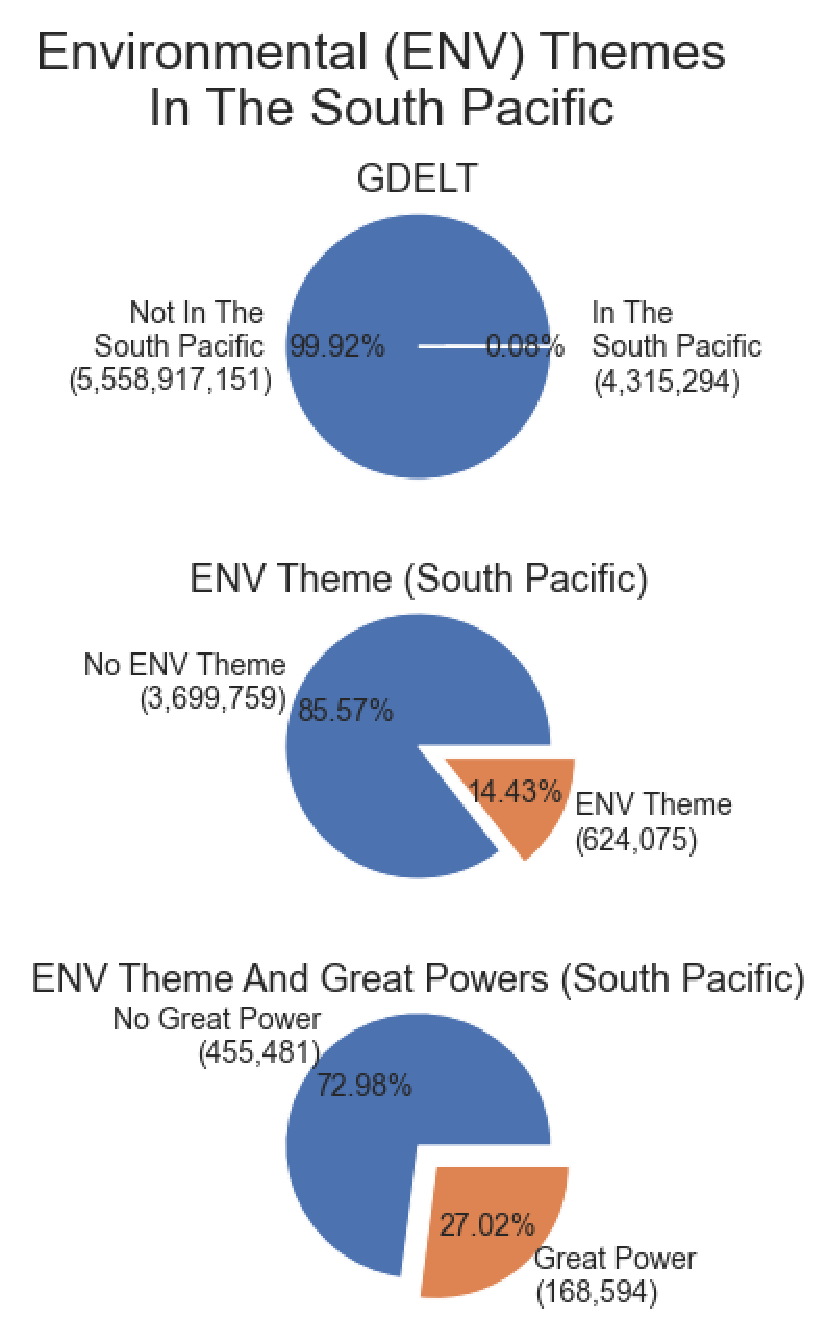
\includegraphics[width=0.5\textwidth]{GDELT Pie}}
\begin{wrapfigure}{R}{0.5\textwidth}
\vspace{-40pt}
  \begin{center}
    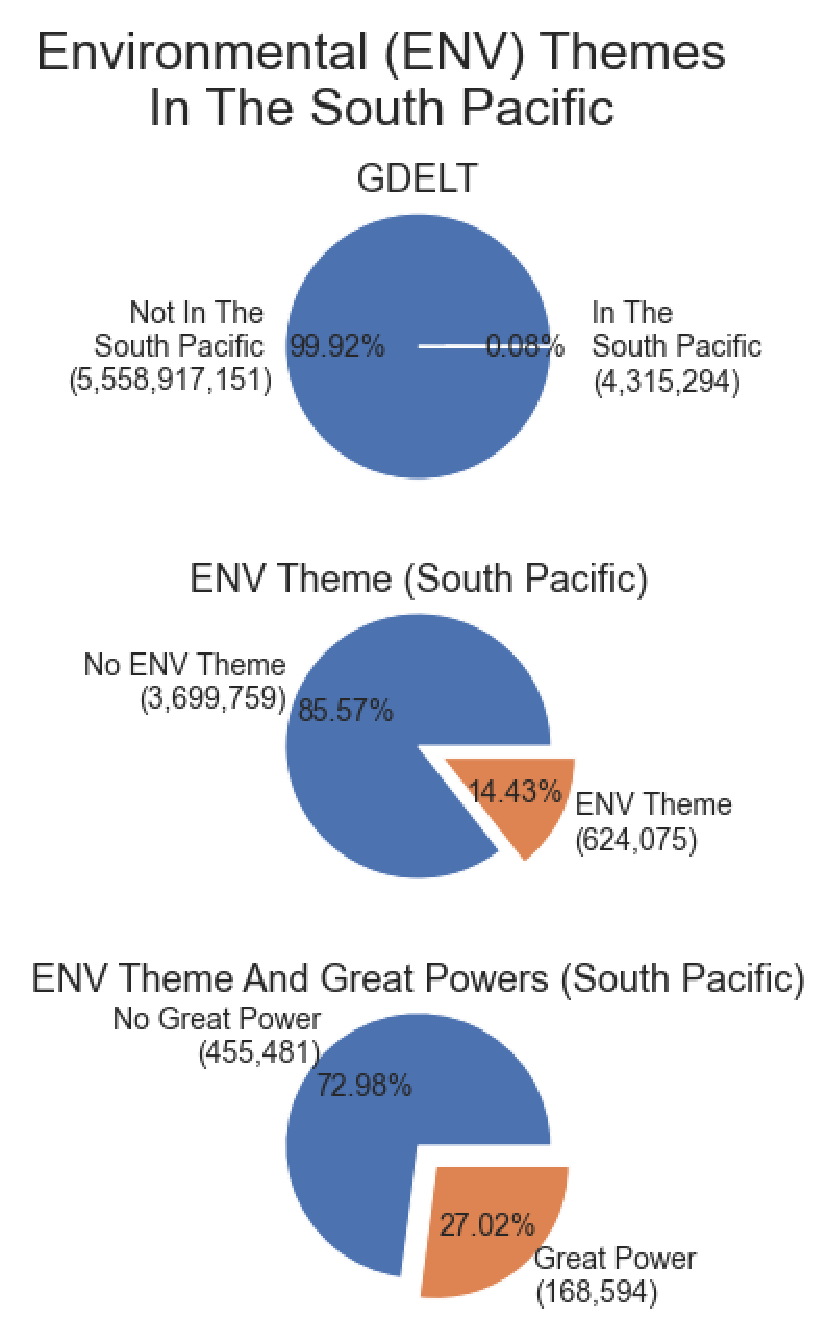
\includegraphics[width=0.5\textwidth]{GDELT Pie}
  \end{center}
  \vspace{-20pt}
  \caption{Breakdown of GDELT}
  \vspace{-60pt}
  \label{fig:mesh1}
\end{wrapfigure}

A further breakdown of the six great powers in the South Pacific, shows that the United States (\textit{USA}) is the top actor with being in over 47\% (48,561) of the articles where a great power is present and the article involves an environmental theme. Next is Australia (\textit{AUS}) with over 17\% (17,919), China (\textit{CHN}) with over 14\% (15,057), New Zealand (\textit{NZL}) with over 11\% (11,228), Japan (\textit{JPN}) with over 7\% (7,919), and Russia \textit{(RUS)} with over 1\% (1,253). [\textit{Figure \ref{fig:mesh2}}]

\section*{Methods}

\subsection*{Identifying Locations in the South Pacific}
To create a subset of data that only contains events in the South Pacific, we had to identify all the location within the South Pacific and there FIPS10-4 country codes. GDELT uses the Federal Information Processing Standards (FIPS) codes to identify each events’ unique location. 
The first place we looked to find all the countries and territories in the South Pacific was Wikipedia because Wikipedia has a list of names of most of the sovereign states and dependent territories in the South Pacific [5]. We also decided to excluded Australia and New Zealand from our initial list of nations to include in our data set because both of those nations are already well developed and are major influences on the many of the nations in the South Pacific. 
After we had a list of countries and territories we wanted to include in our research, we then needed to find each locations corresponding FIPS code. To find each FIPS code, I ran the following query through BigQuery:
\begin{lstlisting}[
           language=SQL,
           showspaces=false,
           basicstyle=\small,
           numbers=left,
           numberstyle=\small,
           commentstyle=\color{gray},
           caption=Getting The List Of Countries And Territories In GDELT
        ]
    SELECT
        Actor1Name, Actor1CountryCode, Actor2Name, Actor2CountyCode, 
        Actor1Geo_FullName Actor1Geo_CountryCode, Actor2Geo_FullName, 
        Actor2Geo_CountryCode, ActionGeo_FullName, ActionGeo_ADM1Code 
    FROM 
        `gdelt-bq.gdeltv2.events` 
\end{lstlisting}

\begin{figure}
	\centering
	\includegraphics[width=\textwidth]{GD Portions}
	\caption{Breakdown of Articles by Great Power}
    \label{fig:mesh2}
\end{figure}

And saved the results into a CSV file. Next, I manually searched the file in Excel for each corresponding locations’ two-digit country code (\textit{ActionGeo\_CountryCode}). I found this method to be the fastest and most precise way of finding each location in the South Pacific compared to other methods like querying for each location in BigQuery or searching other online resources. We could not trust the FIPS codes found on the internet because there were inconsistencies between what GDELT labeled certain territories compared to what was found online.

Using this method, I was successful in identifying almost every region except for the locations of Territory of Ashmore and Cartier Islands, Galápagos Islands, Midway Islands, Ogasawara village, Papua Province, and West Papua. Searching for these locations returned some results that did not seem to match the location within the south pacific or did not return a result at all. I found the names and their country codes within GDELT after querying GDELT itself. I did however initially miss-identify West Papua's \textit{ActionGeo\_ADM1Code} for a different part of Indonesia. I eventually found the correct \textit{ActionGeo\_ADM1Code} for West Papua after a series of queries made against the GDELT data set on BigQuery and using Google maps to confirm the regions. 

\subsection*{ActionGeo\_ADM1Code instead of ActionGeo\_CountryCode}

I decided to use \textit{ActionGeo\_ADM1Code} as the main predicate for filtering by location in the queries ran through BigQuery. There are two reasons that made me decide to use \textit{ActionGeo\_ADM1Code} instead of \textit{ActionGeo\_CountryCode} or \textit{ActionGeo\_FullName} in my query. The first is that I found that when trying to filter a location by explicitly stating the name of the region (\textit{ActionGeo\_FullName}) produced a data set with less articles compared to using the \textit{ActionGeo\_ADM1Code}. For example, I found that when using the filtering by \textit{ActionGeo\_FullName = 'Hawaii, United States'} vs using \textit{ActionGeo\_ADM1Code = 'USHI'}, (At the time of the initial query) there was \textbf{346,532} more articles that were found using \textit{ActionGeo\_ADM1Code = 'USHI'}. The second reason was for consistency in which predicates I was using within the query itself. Because every \textit{ActionGeo\_ADM1Code} is anywhere between 2 and 4 characters and the first two characters of the \textit{ActionGeo\_ADM1Code} are always the same as the \textit{ActionGeo\_CountryCode}. I still capture the same number of articles using \textit{ActionGeo\_ADM1Code} as the predicate as we would using \textit{ActionGeo\_CountryCode}. 

However, some locations within the South Pacific are part of countries that are not entirely considered to be in the South Pacific. For example, Indonesia has two regions that are a part of the South Pacific, but Indonesia itself is not entirely in the South Pacific. To only get those specific regions of Indonesia, I had to explicitly state the whole \textit{ActionGeo\_ADM1Code} for West Papua and Papua. Also, the locations of Ashmore and Cartier Islands falls underneath an \textit{ActionGeo\_ADM1Code} that captures more than just that region. For this reason, I had to explicitly state the regions, using the \textit{ActionGeo\_FullName}, of Ashmore Reef, Queensland, Australia, Coral Sea Islands, Easter Island, the Galapagos Islands, Midway Islands, Ogasawaramura Islands, and the Bonin Islands. 

\subsection*{Joining the Events, Eventmentions, and GKG}

To access all the attributes about each article (Themes and Tone), I had to join the Events, Eventmentions, and GKG table together. The Events and Eventmentions table joined on the \textit{GLOBALEVENTID}'s and the GKG joined to the Eventmentions table through the Eventmentions \textit{MentionIdentifier} is the same as the GKG \textit{DocumentIdentifier}. 
    
When joining all three tables together and using ActionGeo\_ADM1Code as the predicates in the query, the resulting data set produced a table with 4,323,833 entries. When initially filtering which columns to also include in the data set, I decided to pull every column that could be of some relevance for this research. This meant excluding many of the attributes that are in the Events, Eventmentions, and GKG table. Even with excluding most attributes, this still led to a data set that was almost 20 GB (gigabytes) in size. With such a massive data set produced from BigQuery, it presented its own challenges on how to perform certain aggregations and data wrangling. 
    
Because the Pandas library, from Python, embeds the data frame in RAM (Random Access Memory), this meant I could not access more than one instance of this data set at a time. This led to issues when I used the SQLite library using Python to perform queries on the data set. Because SQLite also embeds its data base in memory (instead of the disk drive like a traditional SQL frameworks), I had to load the data set directly into SQLite from Pandas and delete the instance of that data set immediately after it was done to perform queries. To conserve memory within my computer, I eventually made mini data sets of only the attributes used in this research so I could hold both an instance of the data set in Pandas and in SQLite. Doing this allowed me to do data aggregation with SQL and then further analysis using Python without having to drop one instance to use the other. 

However, I was eventually able to only use Python for all my data analysis, including the data wrangling, just from using the Pandas library. This allowed me to pull only the columns I needed from the larger 20GB data set. Which saved how much RAM was being occupied at any given time and improved performance.  

\subsection*{Pandas to Filter Themes}

From the GKG table, the two attributes of interest for this research are the \textit{Themes} and the \textit{Tones}. The \textit{Themes} attribute allowed us to filter our data set of the South Pacific to only contain events that involves the environment. The environmental themes of interest were filtered from the original data set by using Pandas and boolean masks combined with Pythons \textit{str.contains()} method. This allowed us to create a data set that only contained articles where there is an environmental theme associated with it. 

There are 21 different environmental themes that GDELT has created: 
\linebreak
\setlength{\parindent}{0cm}
\textit{ENV\_CLIMATECHANGE}, \textit{ENV\_OIL}, \textit{ENV\_FISHERY}, \textit{ENV\_MINING}, \textit{ENV\_COAL},
\linebreak
\textit{ENV\_GREEN}, 
\textit{ENV\_SOLAR}, \textit{ENV\_METALS}, \textit{ENV\_POACHING}, \textit{ENV\_NATURALGAS}, 
\linebreak
\textit{ENV\_DEFORESTATION}, \textit{ENV\_OVERFISH}, \textit{ENV\_FORESTRY}, \textit{ENV\_NUCLEARPOWER}, \textit{ENV\_WATERWAYS}, \textit{ENV\_SPECIESENDANGERED}, \textit{ENV\_HYDRO}, \textit{ENV\_BIOFUEL}, 
\linebreak
\textit{ENV\_GEOTHERMAL}, \textit{ENV\_WINDPOWER}, \textit{ENV\_CARBONCAPTURE}, and 
\linebreak
\textit{ENV\_SPECIESEXTINCT}. 
\setlength{\parindent}{1cm}


GDELT also has the World Bank themes included in the \textit{Themes} column. The World Bank themes offer even greater details in their themes than what GDELT has provided with its own themes. But for this research, we only are filtering by the themes that begin with \textit{'ENV\_'} because the World Bank themes do not follow a uniform structure. Therefore, making it exceedingly difficult to only filter by a certain kind of World Bank theme. 

\subsection*{V2Themes vs Themes}

Within the GKG table, there are two themes columns. One is labeled \textit{Themes} and the other \textit{V2Themes}. After doing a detailed analysis of both columns, I concluded that both columns produced nearly identical results and choosing one over the other was not important for this research. The major differences between the \textit{Themes} and \textit{V2Themes} is the \textit{V2Themes} states the character offset within the article where the theme was identified. \textit{V2Themes} also allows for the same theme to appear more than once in the column if it appears more than once in the event. The \textit{Themes} is only a list of each unique theme as it appears in the event. For this research, I decided to use \textit{V2Themes} instead of \textit{Themes} when filtering by articles involving the environment. However, we could have used \textit{Themes} instead and gotten the same results for this research. 

\subsection*{Tones}

Even though the Events and Eventmentions tables also has a tone attribute, I wanted to present all three of them in this report. There is a slight difference on how each of the tones are calculated in each table. The tone in the Events (\textit{AvgTone}) table only represents the average tone of all the article that reported the event within the first 15 minutes it was first seen, the Eventmentions tone (\textit{MentionDocTone}) is the tone of each individual article, and the GKG tone (\textit{V2Tone}) is calculated from taking the average of the positive and negative score of the whole document [3][4]. The tones, and positive and negative scores are automatically generated by GDELT using sentiment analysis. The exact algorithms are not mentioned but GDELT promises that it is an advance Natural Language Processing (NLP) algorithm that generates these scores [4][6].

\subsection*{Great Powers}

There is two ways that we can specify when looking for articles only involving the great powers of interest. The first way is by looking for the \textit{Actor1/2CountryCodes} and the other is the \textit{Actor1/2Geo\_CountryCode}. While the \textit{ActorGeo\_CountryCode} method uses the FIPS country codes to specify who the actors are, the attribute \textit{Actor1CountryCode} (and \textit{Actor2CountryCode}) uses a 3-character CAMEO code for the country affiliations. There are resources online to find the \textit{Actor1/2CountryCode} of each of the countries we are looking for. Instead of turning to the internet, I searched the data sets I had already created using Pandas functions. This way, I was able to get the exact \textit{Actor1/2CountryCode}'s for each of the great powers. 
    
I decided to use the \textit{Actor1/2CountryCode} instead of \textit{ActorGeo\_CountryCode} for filtering the data set to only containing the great powers because when analyzing the results of using both, using \textit{Actor1/2Geo\_CountryCode} for specifying an actor produced a data set with less than half of the articles compared to using the \textit{Actor1/2CountryCode}. The Events table in GDELT only specifies two actors and a location. So, if multiple actors are present, GDELT will either leave the field blank or will choose which actors take precedence in the article and assign those actors to those attributes [4]. But the \textit{Actor1/2CountryCodes} do not always match. For instance, "if the text refers to 'French Assistant Minister Smith was in Moscow', the CountryCode field will list France in the CountryCode field, while the geographic fields may list Moscow as the location"[4]. While this leads to potentially missing some articles involving certain actors, if we were to look for actors by either there location (\textit{ActorGeo\_CountryCode}) or there precedence in the article (\textit{ActorCountryCode}), we may be including articles where we have an actors location who maybe was not an actor in the article itself. On the other hand, when specifying having the\textit{ Actor1/2CountryCode} and ActorGeo\_CountryCode matching, only produced a data set that only contained a fraction of the number of events (ten's of thousands compared to hundred's of thousands). 

\subsection*{Media Sources}

\begin{wrapfigure}[21]{r}{0.5\textwidth}
\vspace{-70pt}
  \begin{center}
    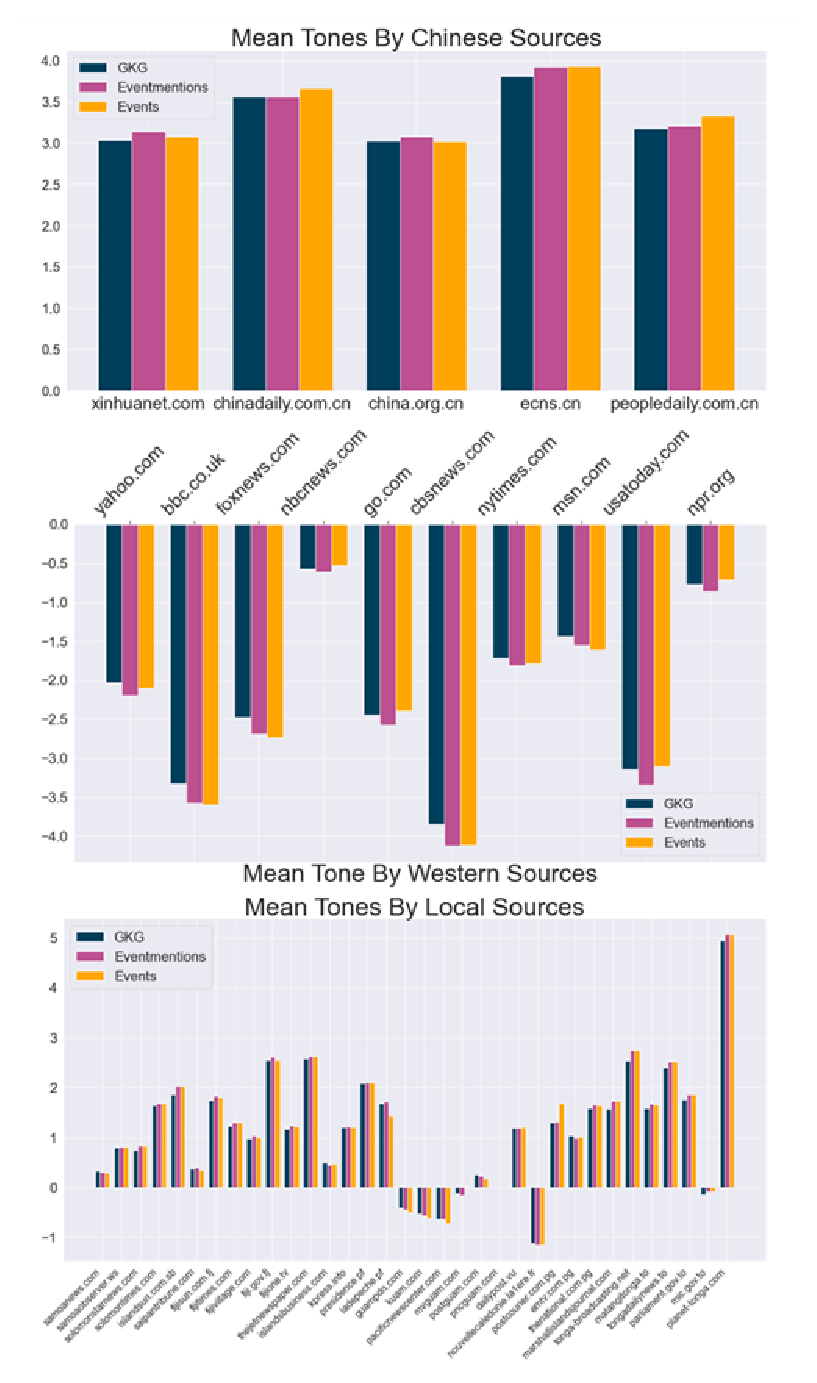
\includegraphics[width=0.5\textwidth]{3 Graphs.eps}
  \end{center}
  \vspace{-20pt}
  \caption{Tones by Sources}
  \vspace{-20pt}
  \label{fig:3Graphs}
\end{wrapfigure}

When finding the Local media sources of the South Pacific, I created a function in Python to output every unique media source that has involves a great power as \textit{Actor1} or \textit{Actor2}. From there, my research mentor (\textit{Dr. Elizabeth Gooch}) went through the list of sources for each individual location and cross checked each source to see if it was a local source. The Western news sources were selected because they give a range of liberal, conservative, and neutral media outlets. The Chinese news sources were select because each one of those news sources are either state-owned, state-ran, or authorized by the Chinese government. 

\subsection*{Calculating Tones}

Once I had the geographical locations, the CAMEO codes for each great power, and the proper filtering methods for creating subsets of data, I then created multiple Python functions to compute the average weighted tone for each news source in the South Pacific [\textit{Figure \ref{fig:3Graphs}}].

\section*{Results}

When comparing each of the three media sources (Chinese, Local, and Western) side by side, Chinese sources have an average tone of around 3.2, Local sources have an average tone of around 0.7, and Western sources have an average tone of 1.8-1.9. The tones in GDELT can have a score of +100 to -100 but most of the tone scores are between +10 and -10 (where -10 is an article written with a very negative sentiment, +10 is written with a very positive sentiment, and 0 indicating neutral) [4][\textit{Figure \ref{fig:mesh4}}].

\begin{figure}[H]
	\centering
	\includegraphics[width=\textwidth]{Results.eps}
	\caption{Mean Tones By Source}
    \label{fig:mesh4}
\end{figure}

\subsection*{Difference In Means}

In order to prove each of the population means are statistically significance, I conducted a difference in means tests for each of our three sources. For the rest of the report, I conducted my statistical analysis using R. I did this for a few reasons. One, R has better interpret-ability with the results. In Python, similar functions used to conducted statistical analysis using the SciPy library usually produce only single number results. To show the results in a presentable manor, I would need to create additional functions with print statements explaining the results of each test. Instead of doing this, I decided R would be the better choice. Two, the data visualizations produced in R using \textit{ggplot} and \textit{base R} produce very clean graphics with minimal amount of coding compared to Python. I still however used Python for all the data aggregation and pre-processing of the data set and then imported it into R for the data visualizations and statistical analysis.

In order to prepare the data for statistical analysis using R, I filtered the data set one more time to only contain the \textit{GKG\_Tone} and added a new column to indicated if the \textit{Source} was a Chinese source, Local source, or Western Source.

To conduct a difference in means test, we must acknowledge the assumptions to conduct this statistical analysis. First, we will assume that each observation from each of the groups are independent of each other group. Next, I checked the normality by creating three distribution plots and a Q-Q plot [\textit{Figure \ref{fig:Normality}}, \ref{fig:Distributions}]. This showed that the data overall follows a normal distribution.\renewcommand{\thefootnote}{\roman{footnote}}\footnote{Because the number of observations is large (Chinese = 1,013, Local = 10,292, Western = 3,348), violating the normality assumption is okay.} Finally, when checking for equal variances in the Residuals vs Fitted plot, the variances appeared to not be equal among the three groups [\textit{Figure \ref{fig:Normality}}]. Because of this inconsistency, I conducted a Levene Test in R to test the homogeneity of variances of the residuals.

\begin{figure}
	\centering
	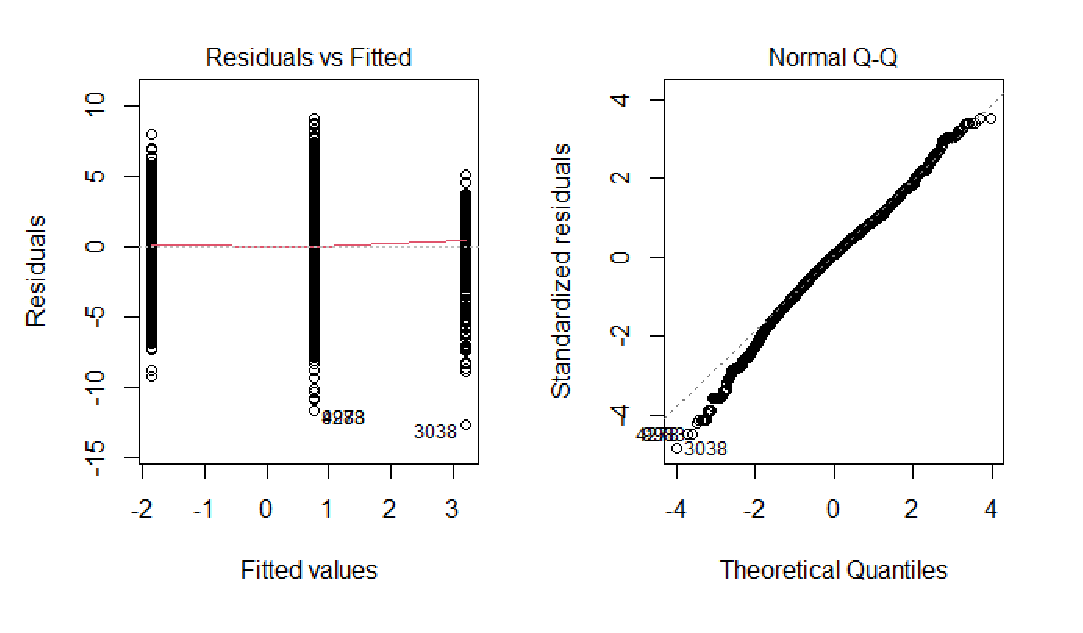
\includegraphics[width=\textwidth]{Normality R.eps}
	\caption{Normality and Variance of Tones}
    \label{fig:Normality}
\end{figure}

\begin{figure}
	\centering
	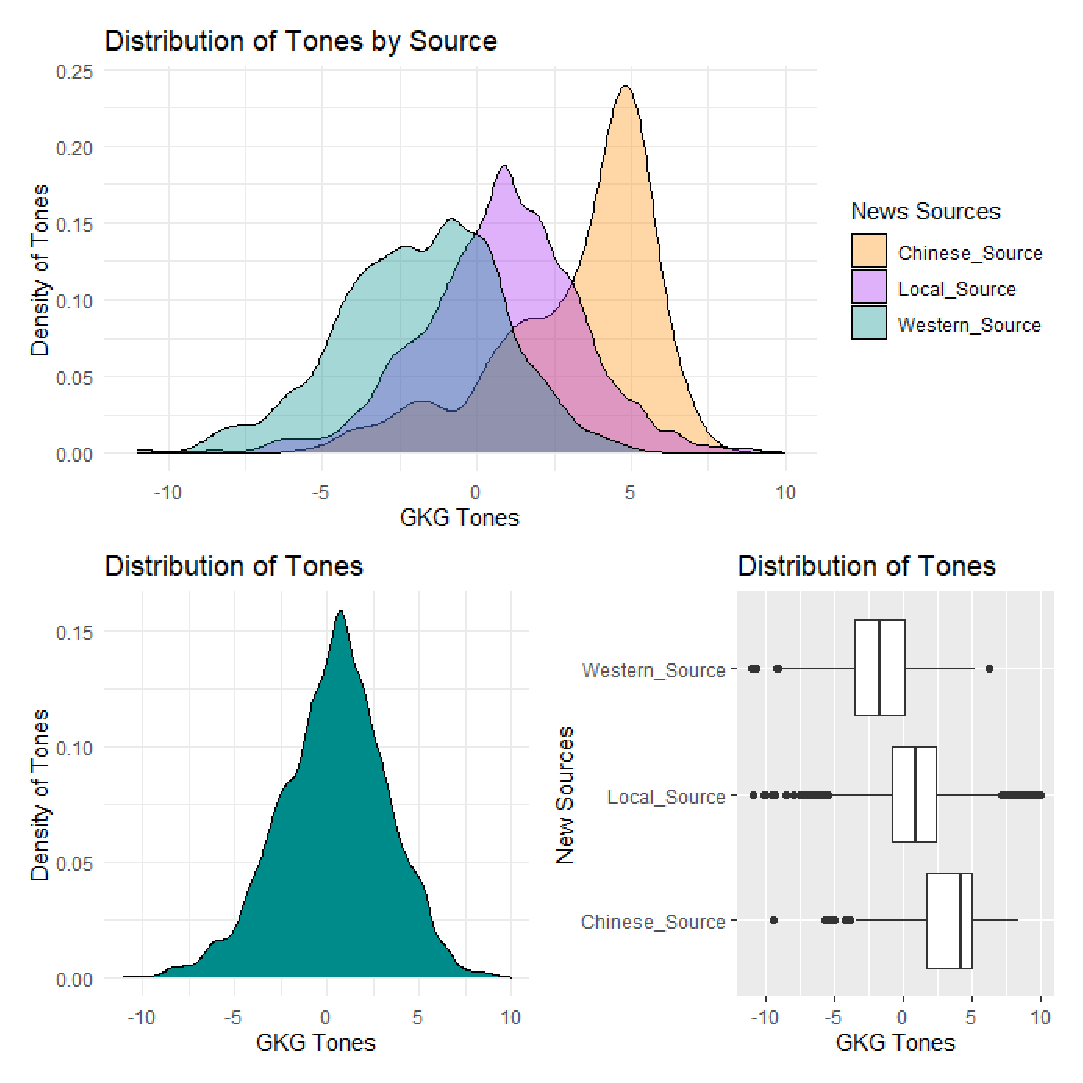
\includegraphics[width=\textwidth]{Distribution of Tones GDELT.eps}
	\caption{Normality of Tones}
    \label{fig:Distributions}
\end{figure}

\begin{lstlisting}[language=R,
                    frame=single,
                    basicstyle=\small\ttfamily,
                    stringstyle=\color{DarkGreen},
                    otherkeywords={0,1,2,3,4,5,6,7,8,9},
                    morekeywords={TRUE,FALSE},
                    deletekeywords={data,frame,length,as,character},
                    keywordstyle=\color{None},
                    commentstyle=\color{DarkGreen},
                    showspaces=False,
                    showstringspaces=false,
                    caption= Levene's Test for Homogeneity of Variance,
                    label={lst:R_code_1}]
> tones <- read_csv('source_tones.csv')
> leveneTest(GKG_Tone ~ Source, data=tones)
Levene's Test for Homogeneity of Variance (center = median)
         Df F value    Pr(>F)    
group     2  7.5008 0.0005548 ***
      14650                      
---
Signif. codes: 0 `***` 0.001 `**` 0.01 `*` 0.05 `.` 0.1 ` ` 1
\end{lstlisting}

To interpret the results of the Levene's Test for Homogeneity of Variance, at a confidence level of $\alpha$ = 0.05 and p-value of 0.0005, we conclude that the population variances are not equal.  

Because the population variances are not equal, we will need to conducted three Welch's t-test's for each of the pairwise groups .\renewcommand{\thefootnote}{\roman{footnote}}\footnote{Group 1: Local Sources - Chinese Sources, Group 2: Western Sources - Chinese Sources, Group 3: Western Sources - Local Sources} 

\begin{lstlisting}[Language=R,
                    frame=single,
                    basicstyle=\small\ttfamily,
                    stringstyle=\color{DarkGreen},
                    otherkeywords={0,1,2,3,4,5,6,7,8,9},
                    morekeywords={TRUE,FALSE},
                    deletekeywords={data,frame,length,as,character},
                    keywordstyle=\color{None},
                    commentstyle=\color{DarkGreen},
                    showspaces=False,
                    showstringspaces=false,
                    caption= Pairwise Comparisons for Tones,
                    label={lst:R_code_2}]
> data.local <- subset(tones, Source == "Local_Source")
> data.western <- subset(tones, Source == "Western_Source")
> data.chinese <- subset(tones, Source == "Chinese_Source")
> ### Local_Source-Chinese_Source
> t.test(data.local$GKG_Tone, data.chinese$GKG_Tone,
+        mu=0, alternative="two.sided", 
+        var.equal = FALSE) 

	Welch Two Sample t-test

data:  data.local$GKG_Tone and data.chinese$GKG_Tone
t = -28.536, df = 1218.7, p-value < 2.2e-16
alternative hypothesis: true difference in means is not equal to 0
95 percent confidence interval:
 -2.610919 -2.275004
sample estimates:
mean of x mean of y 
0.7589979 3.2019597 

> ### Western_Source-Chinese_Source
> t.test(data.western$GKG_Tone, data.chinese$GKG_Tone,
+        mu=0, alternative="two.sided", 
+        var.equal = FALSE) 

	Welch Two Sample t-test

data:  data.western$GKG_Tone and data.chinese$GKG_Tone
t = -53.947, df = 1684.2, p-value < 2.2e-16
alternative hypothesis: true difference in means is not equal to 0
95 percent confidence interval:
 -5.225113 -4.858498
sample estimates:
mean of x mean of y 
-1.839846  3.201960 

> ### Western_Source-Local_Source
> t.test(data.western$GKG_Tone, data.local$GKG_Tone,
+        mu=0, alternative="two.sided", 
+        var.equal = FALSE) 

	Welch Two Sample t-test

data:  data.western$GKG_Tone and data.local$GKG_Tone
t = -49.899, df = 5624.3, p-value < 2.2e-16
alternative hypothesis: true difference in means is not equal to 0
95 percent confidence interval:
 -2.700946 -2.496742
sample estimates:
 mean of x  mean of y 
-1.8398457  0.7589979 
\end{lstlisting}

\subsection*{Interpreting Welch two-samples t-test's}

After conducting these tests in R, we show that the difference in means between each pairwise group is statistically significant. 

\subsubsection*{Local Sources and Chinese Sources}

The Welch two-samples t-test between Local Sources and Chinese Sources showed that the difference is statistically significant, t = -28.536, df = 1218.7, p-value < 2.2e-16. 

\subsubsection*{Western Sources and Chinese Sources}

The Welch two-samples t-test between Western Sources and Chinese Sources showed that the difference is statistically significant, t = -53.947, df = 1684.2, p-value < 2.2e-16.

\subsubsection*{Western Sources and Local Sources}

The Welch two-samples t-test between Western Sources and Chinese Sources showed that the difference is statistically significant, t = -49.899, df = 5624.3, p-value < 2.2e-16.

\section*{Conclusion}

In this report, I introduce GDELT and how GDELT can be used to track events in regions of the world. I talked about the three tables (Events, Eventmentions, GKG) we used in this research, how they all relate, and which attributes were important for this research. I showed how I found the exact locations and actors within GDELT using GDELT itself and Wikipedia. I mentioned which countries and territories we included in this research and some that we did not. I showed the queries used to pull our data set from BigQuery. I showed the number of articles within GDELT that have an event located in the South Pacific only accounts for 0.08\% of the articles within GDELT itself, of the 4.32 million articles in our data set, only 14.43\% involve an environmental theme, and when a great power was an actor in an event in the South Pacific, 27.02\% of those events had an environmental theme. 

Next, I showed all the methods I used to develop our final data set. I gave explanations on which attributes I decided to choose for our filtering and how I used Python for all of my data wrangling, exploration, and most of the visualizations. I explained why we chose our media sources and how I calculated our average tones for each source. I then showed that Chinese sources have an overall very positive tone in the South Pacific when the event itself involves the environment, Local news sources have a positive to neutral tone, and Western sources have a negative tone. And finally, I proved (using R) the mean tones of Chinese, Local, and Western new sources are statistically different.

\section*{Acknowledgment}

I would like to thank Dr. Elizabeth Gooch from the Naval Postgraduate School for mentoring me and the Undergraduate Research Opportunity Center (UROC) Program at California State University, Monterey Bay for providing me a scholarship for this research.



\pagestyle{plain}

\begin{thebibliography}{}

\bibitem{1} 
https://www.gdeltproject.org/about.html

\bibitem{2} 
https://www.gdeltproject.org/ 

\bibitem{3} 
http://data.gdeltproject.org/documentation/GDELT-Global\_Knowledge\_Graph\_Codebook-V2.1.pdf

\bibitem{4}
http://data.gdeltproject.org/documentation/GDELT-Event\_Codebook-V2.0.pdf

\bibitem{5} 
https://en.wikipedia.org/wiki/Oceania

\bibitem{6} 
https://blog.gdeltproject.org/introducing-gkg-2-0-the-next-generation-of-the-gdelt-global-knowledge-graph/

\end{thebibliography}

\end{document}
